%!TEX program = xelatex
\documentclass[cn,black,12pt,normal]{elegantnote}
\usepackage{float}
\usepackage{hyperref}
\usepackage{amsmath}
\usepackage{amsfonts}
\usepackage{amssymb}
\usepackage{siunitx}[=v2]
\usepackage{fancyhdr}
\usepackage{newtxtext}
\usepackage{algorithm}
\usepackage{algorithmic}
\newcommand{\uct}[1]{\textsuperscript{\textsuperscript{\cite{#1}}}}
\renewcommand{\tablename}{\textbf{Table}}
\renewcommand{\figurename}{Figure.}
\renewcommand{\refname}{References}
\renewcommand{\contentsname}{Contents}
\renewcommand{\versiontext}{Version: }
\renewcommand{\updatetext}{Update: }
\PassOptionsToPackage{no-math}{fontspec}
\lstset{basicstyle=\footnotesize\ttfamily\color[RGB]{50,0,130},numbers=none,frame=trBL}

\sisetup{mode=text}
\sisetup{range-phrase = \text{ \textasciitilde }}
\pagestyle{fancy}
\fancyhead[L]{School of Software Engineering, Tongji University}
\fancyhead[R]{Data Structure Projects}
\renewcommand{\headrulewidth}{1pt}

\title{Data Structure Projects\\Overview}
\author{姜文渊}
\institute{School of Software Engineering, Tongji University}
\version{0.50}
\date{\today}

\begin{document}

\maketitle

\section{Introduction}

In the data structure project of this semester, the author completed the tasks required by the course, which are listed below.

\begin{enumerate}
    \item Exam Registration System (考试报名系统)
    \item Joseph Game (约瑟夫生者死者游戏)
    \item Maze Game (勇闯迷宫游戏)
    \item N-Queen Problem (N皇后问题)
    \item Keyword Search (关键字检索系统)
    \item Family Tree (家谱管理系统)
    \item Expression Eval (表达式计算)
    \item Electric Network (电网建设造价模拟系统)
    \item Binary Sort Tree (二叉排序数)
    \item Sort Algorithms (8种排序算法的比较案例)
\end{enumerate}

The solution of each task meets the requirements given by the course, and more work has been done to make the solutions more user-friendly and more robust. Detailed demostration will be shown in the following documents, which contains the usage of each solution, the algorithms and math behind the solutions, and related analysis.

In this \lstinline{README}, the author will show the general structure of the code, together with the development environment of this project and the ways to build the solutions. All the code and the commit history of this project will be found on \url{https://github.com/jwyjohn/Jwy_DataStructureHomework}.

\section{Structure of the project}

In the root folder of the git repo, dirctories named like \lstinline{10_Sort} can be found. One example of the structure of these dirctories is shown below.

\begin{lstlisting}
10_Sort/
|-- 10_1951510_姜文渊.cpp
|-- 10_1951510_姜文渊.exe
`-- linux
    |-- Makefile
    |-- sort.cpp
    `-- sort.h
1 directory, 5 files
\end{lstlisting}

As can be seen, one \lstinline{*.cpp} file and one \lstinline{*.exe} file can be found. They are the source file and its compiled corresponding windows executable. If the windows executable won't run properly on your windows platform (which is a rare situation), then it is recommended to recompile the source file on your platform.

The \lstinline{linux} dirctory holds several files: \lstinline{*.cpp}, \lstinline{*.h}, \lstinline{Makefile} and two more text files. The header and source file are to be compiled using the configurations provided in \lstinline{Makefile}. Since there are no binary provided, you may need to compiled the files on your own linux distribution.


\section{How to build}

Since the author follows the Minimalism principles, under normal circumstances a C++ compiler which supports the C++ 11 standard with common library properly configured will smoothly compile the project. However, on some special platforms like \lstinline{PowerPC} or \lstinline{arm64}, subtle problems may occure, and the author dose not tested the solutions on those platforms.

Following are the typical ways of compiling a project solution.

\subsection{On Windows}

\begin{figure}[H]
    \centering
    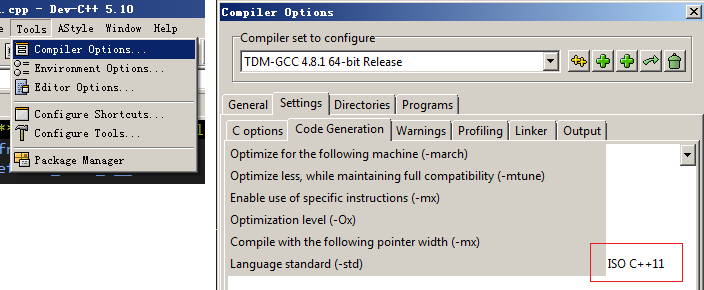
\includegraphics[width=1.0\linewidth]{image/dev02.png}
    \caption{Change Language Standard to C++ 11 in DevC++}
\end{figure}

\begin{enumerate}
    \item Download \lstinline{DevC++ 5.11}
    \item Open the \lstinline{.\*.cpp} with \lstinline{DevC++}
    \item In \lstinline{[Tools]->[Compiler Options...]}, change \lstinline{[Settings]->[Code Generation]->[Language Standard (-std)]} to \lstinline{ISO C++ 11}
    \item Press \lstinline{F10} to compile and run
\end{enumerate}



\subsection{On Linux}

\begin{enumerate}
    \item Check you have installed \lstinline{g++} and \lstinline{make}
    \item Check the environment virables in \lstinline{./Linux/Makefile} and modify them if necessary
    \item (in a shell) Change dirctory to \lstinline{./Linux/} using \lstinline{cd ./Linux}
    \item Run \lstinline{make build} to build
    \item Run the binary generated in the dirctory
    \item Use \lstinline{make clean} to remove temp files and the binary
\end{enumerate}

\section{About the development platform}

The author tested the projects on an \lstinline{x86_64} machine with \lstinline{Manjaro Linux} and \lstinline{Windows 7} installed as OS. More detailed information can be found below.

\begin{lstlisting}
-------------------
OS: Linux x86_64
Kernel: 5.10.70-1-MANJARO
Uptime: 8 hours, 28 mins
Shell: bash 5.1.8
Resolution: 1536x864
Terminal: /dev/pts/0
CPU: Intel i3-10105 (8) @ 4.400GHz
GPU: Intel CometLake-S GT2 [UHD Graphics 630]
Memory: 867MiB / 15850MiB

GCC Version:
$ g++ -v
Using built-in specs.
COLLECT_GCC=g++
COLLECT_LTO_WRAPPER=/usr/lib/gcc/x86_64-pc-linux-gnu/11.1.0/lto-wrapper
Target: x86_64-pc-linux-gnu
Configured with: /build/gcc/src/gcc/configure --prefix=/usr --libdir=/usr/lib --libexecdir=/usr/lib --mandir=/usr/share/man --infodir=/usr/share/info --with-bugurl=https://bugs.archlinux.org/ --enable-languages=c,c++,ada,fortran,go,lto,objc,obj-c++,d --with-isl --with-linker-hash-style=gnu --with-system-zlib --enable-__cxa_atexit --enable-cet=auto --enable-checking=release --enable-clocale=gnu --enable-default-pie --enable-default-ssp --enable-gnu-indirect-function --enable-gnu-unique-object --enable-install-libiberty --enable-linker-build-id --enable-lto --enable-multilib --enable-plugin --enable-shared --enable-threads=posix --disable-libssp --disable-libstdcxx-pch --disable-libunwind-exceptions --disable-werror gdc_include_dir=/usr/include/dlang/gdc
Thread model: posix
Supported LTO compression algorithms: zlib zstd
gcc version 11.1.0 (GCC)

\end{lstlisting}

\section{Notes on the source code}

The projects are coded in a non-object-oriented way, since these projects are mostly demos for showing the author's mastery on the data structures. Thus, the C++ template-based programming features (which are often seen in our textbook) are not commonly used, since these demos do not need to be reused. Another reason for not adopting the OOP is that this project is not a group work, and the work can be maintained by a single person, so Encapsulation and Abstraction is not necessary.

You may also find that in the \lstinline{*.cpp} or \lstinline{*.h} files, a \textit{Single-header library for writing CLI applications in C/C++} named \lstinline{libcmdf.h} is inlined into them, adding several hundreds of lines to each file. The implementation of the input and output processing of each demo is done using the \lstinline{libcmdf.h} from \url{https://github.com/ronen25/libcmdf}, for its Cross-platform feature and its relatively small size.

Although the author tried to worte the documents and the code in English to reach a wider audience and getting more remarks on the coding, some of the comments are still in Chinese, which may cause some trouble to non-native Chinese speakers.

\end{document}
